\documentclass[10pt]{beamer}


\mode<presentation> 
{
  \usetheme{Diku}
  \beamertemplatenavigationsymbolsempty
  \setbeamercovered{invisible}
%  \setbeamercovered{transparent}
}



% \mode<presentation> 
% { \usetheme[nat,dogma]{Frederiksberg} }

% \usepackage[danish]{babel}
\usepackage[latin1]{inputenc}
\usepackage{times}
\usepackage[T1]{fontenc}
\usepackage[english]{babel}
\usepackage{hyperref}
\usepackage{animate}
%\usepackage{multimedia}
\usepackage{francois-preamble}
\usepackage{multirow}

\usepackage{multirow}
%\usepackage{movie15}

\newcommand{\cc}{{c\!\!,}}
\newcommand{\degr}[1]{{{#1}^\circ}}

\title{Vision and Image Processing:\\ Camera Models, Homographies}

\author[S. Olsen] % (optional, use only with lots of authors)
{S�ren Olsen}

\institute[DIKU] % (optional, but mostly needed)
{
  Department of Computer Science\\
  University of Copenhagen
}

\date[2014-15 B2] % (optional, should be abbreviation of conference name)
% {Research Presentation, Diku 2006}


% Insert page numbers
\pagenumbering{arabic}
\setbeamertemplate{footline}{\hspace{5pt}\insertpagenumber\vspace{10pt}}



\definecolor{gold}{rgb}{0.95,0.83,0.0}
\definecolor{orange}{rgb}{0.95,0.7,0.0}
% \definecolor{backblue}{rgb}{0.93,0.94,0.99}
\definecolor{backblue}{rgb}{0.95,0.94,0.99}
\definecolor{darkgreen}{rgb}{0.0,0.30,0.0} 

\setbeamercolor*{background canvas}{bg=backblue} 



\newcommand{\myemph}[1]{{\color{blue}{#1}}}
\newcommand{\intrg}[1]{\int_{{#1}=-\infty}^\infty}
\newcommand{\intRR}{\int_{-\infty}^\infty}

\AtBeginSection[]
{
  \begin{frame}<beamer>{Outline}
    \tableofcontents[currentsection,currentsubsection]
  \end{frame}
}

\begin{document}
\maketitle

% would be cool with more images showing applications


%-------------------------------------------------------------------
%   Start slides
%-------------------------------------------------------------------


%----------------------------------------------
\begin{frame}
  \frametitle{Plan for today}
  \begin{itemize}
  \item Introduction to Camera Models, specifically the pinhole model
     and the perspective transformation \\[3mm]
%   \item Vanishing points and vanishing lines \\[3mm]
  \item Homogeneous coordinates,  Homographies \\[3mm]
  \item Camera matrices and parameters
%  \item Midway evaluation
  \item Camera calibration
%  \item Epipolar line geometry, stereo
%   \item Assignment 4
  \end{itemize}
\end{frame}





% ----------------------------------------------------
\begin{frame}
  \frametitle{Cameras and projections}
  \begin{center}
    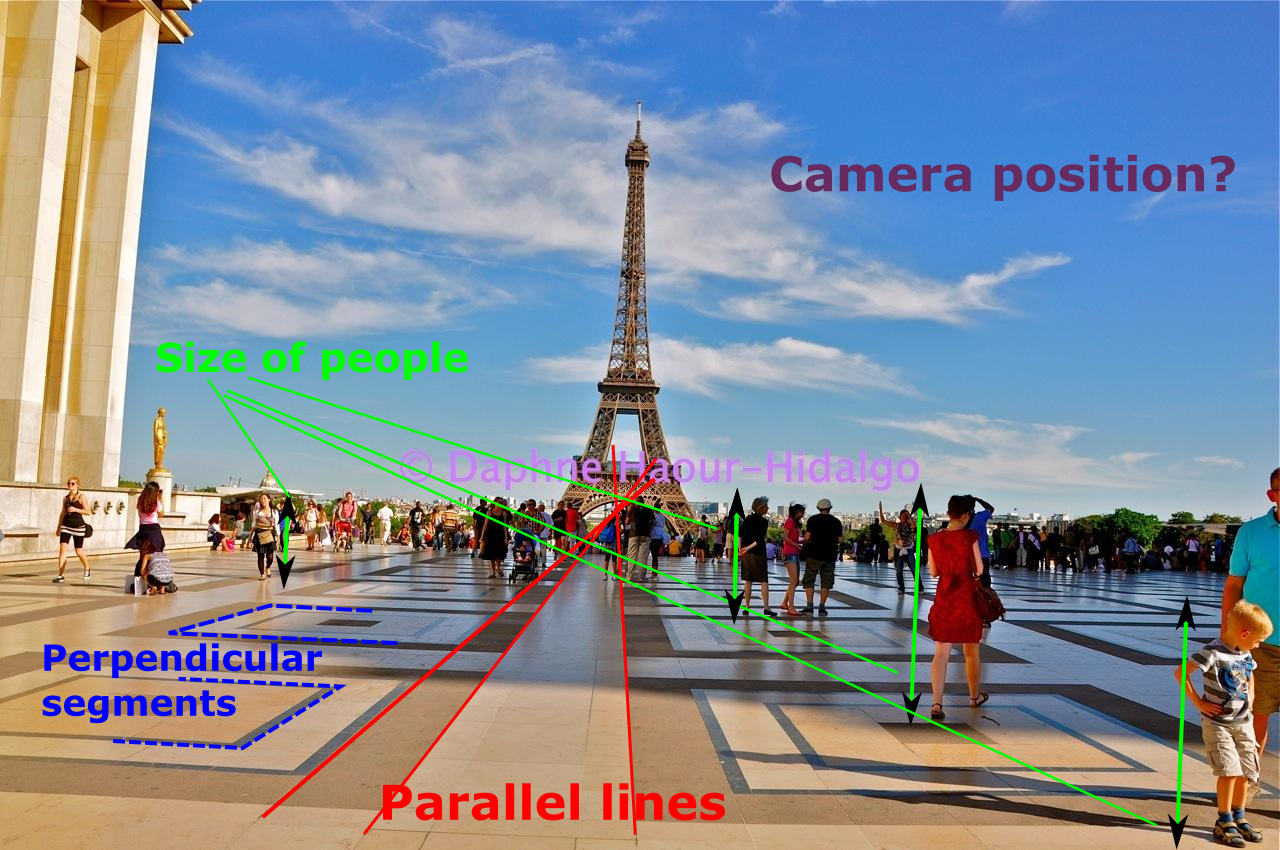
\includegraphics[width=\textwidth]{IMAGES/trocadero_annotations}
  \end{center}
\end{frame}


% ----------------------------------------------------
\begin{frame}
 \frametitle{Questions}
 Previous picture raises some questions about:\vfill
 \begin{itemize}
  \item Lines?
  \item Parallelism?
  \item Angles / orthogonality?
  \item Sizes?
  \item Camera position / Horizon?\vfill
  \end{itemize}
%   What happens when you take a picture (or Daphn{\'e} Haour-Hidalgo in the previous case :-))
\end{frame}


% \section{The Pinhole Camera}


% ----------------------------------------------------
% \begin{frame}
%  \frametitle{Getting an Image -- I}
%  \begin{center}
%    \includegraphics[width=0.55\textwidth]{FIGURES/oliphantnopinhole}
%  \end{center}
%  Many rays emanating from the same position touch the image sensitive
%  array at many location: big blur!
% \end{frame}

% ----------------------------------------------------
% \begin{frame}
%  \frametitle{Getting an Image -- II}
%  \begin{center}
%    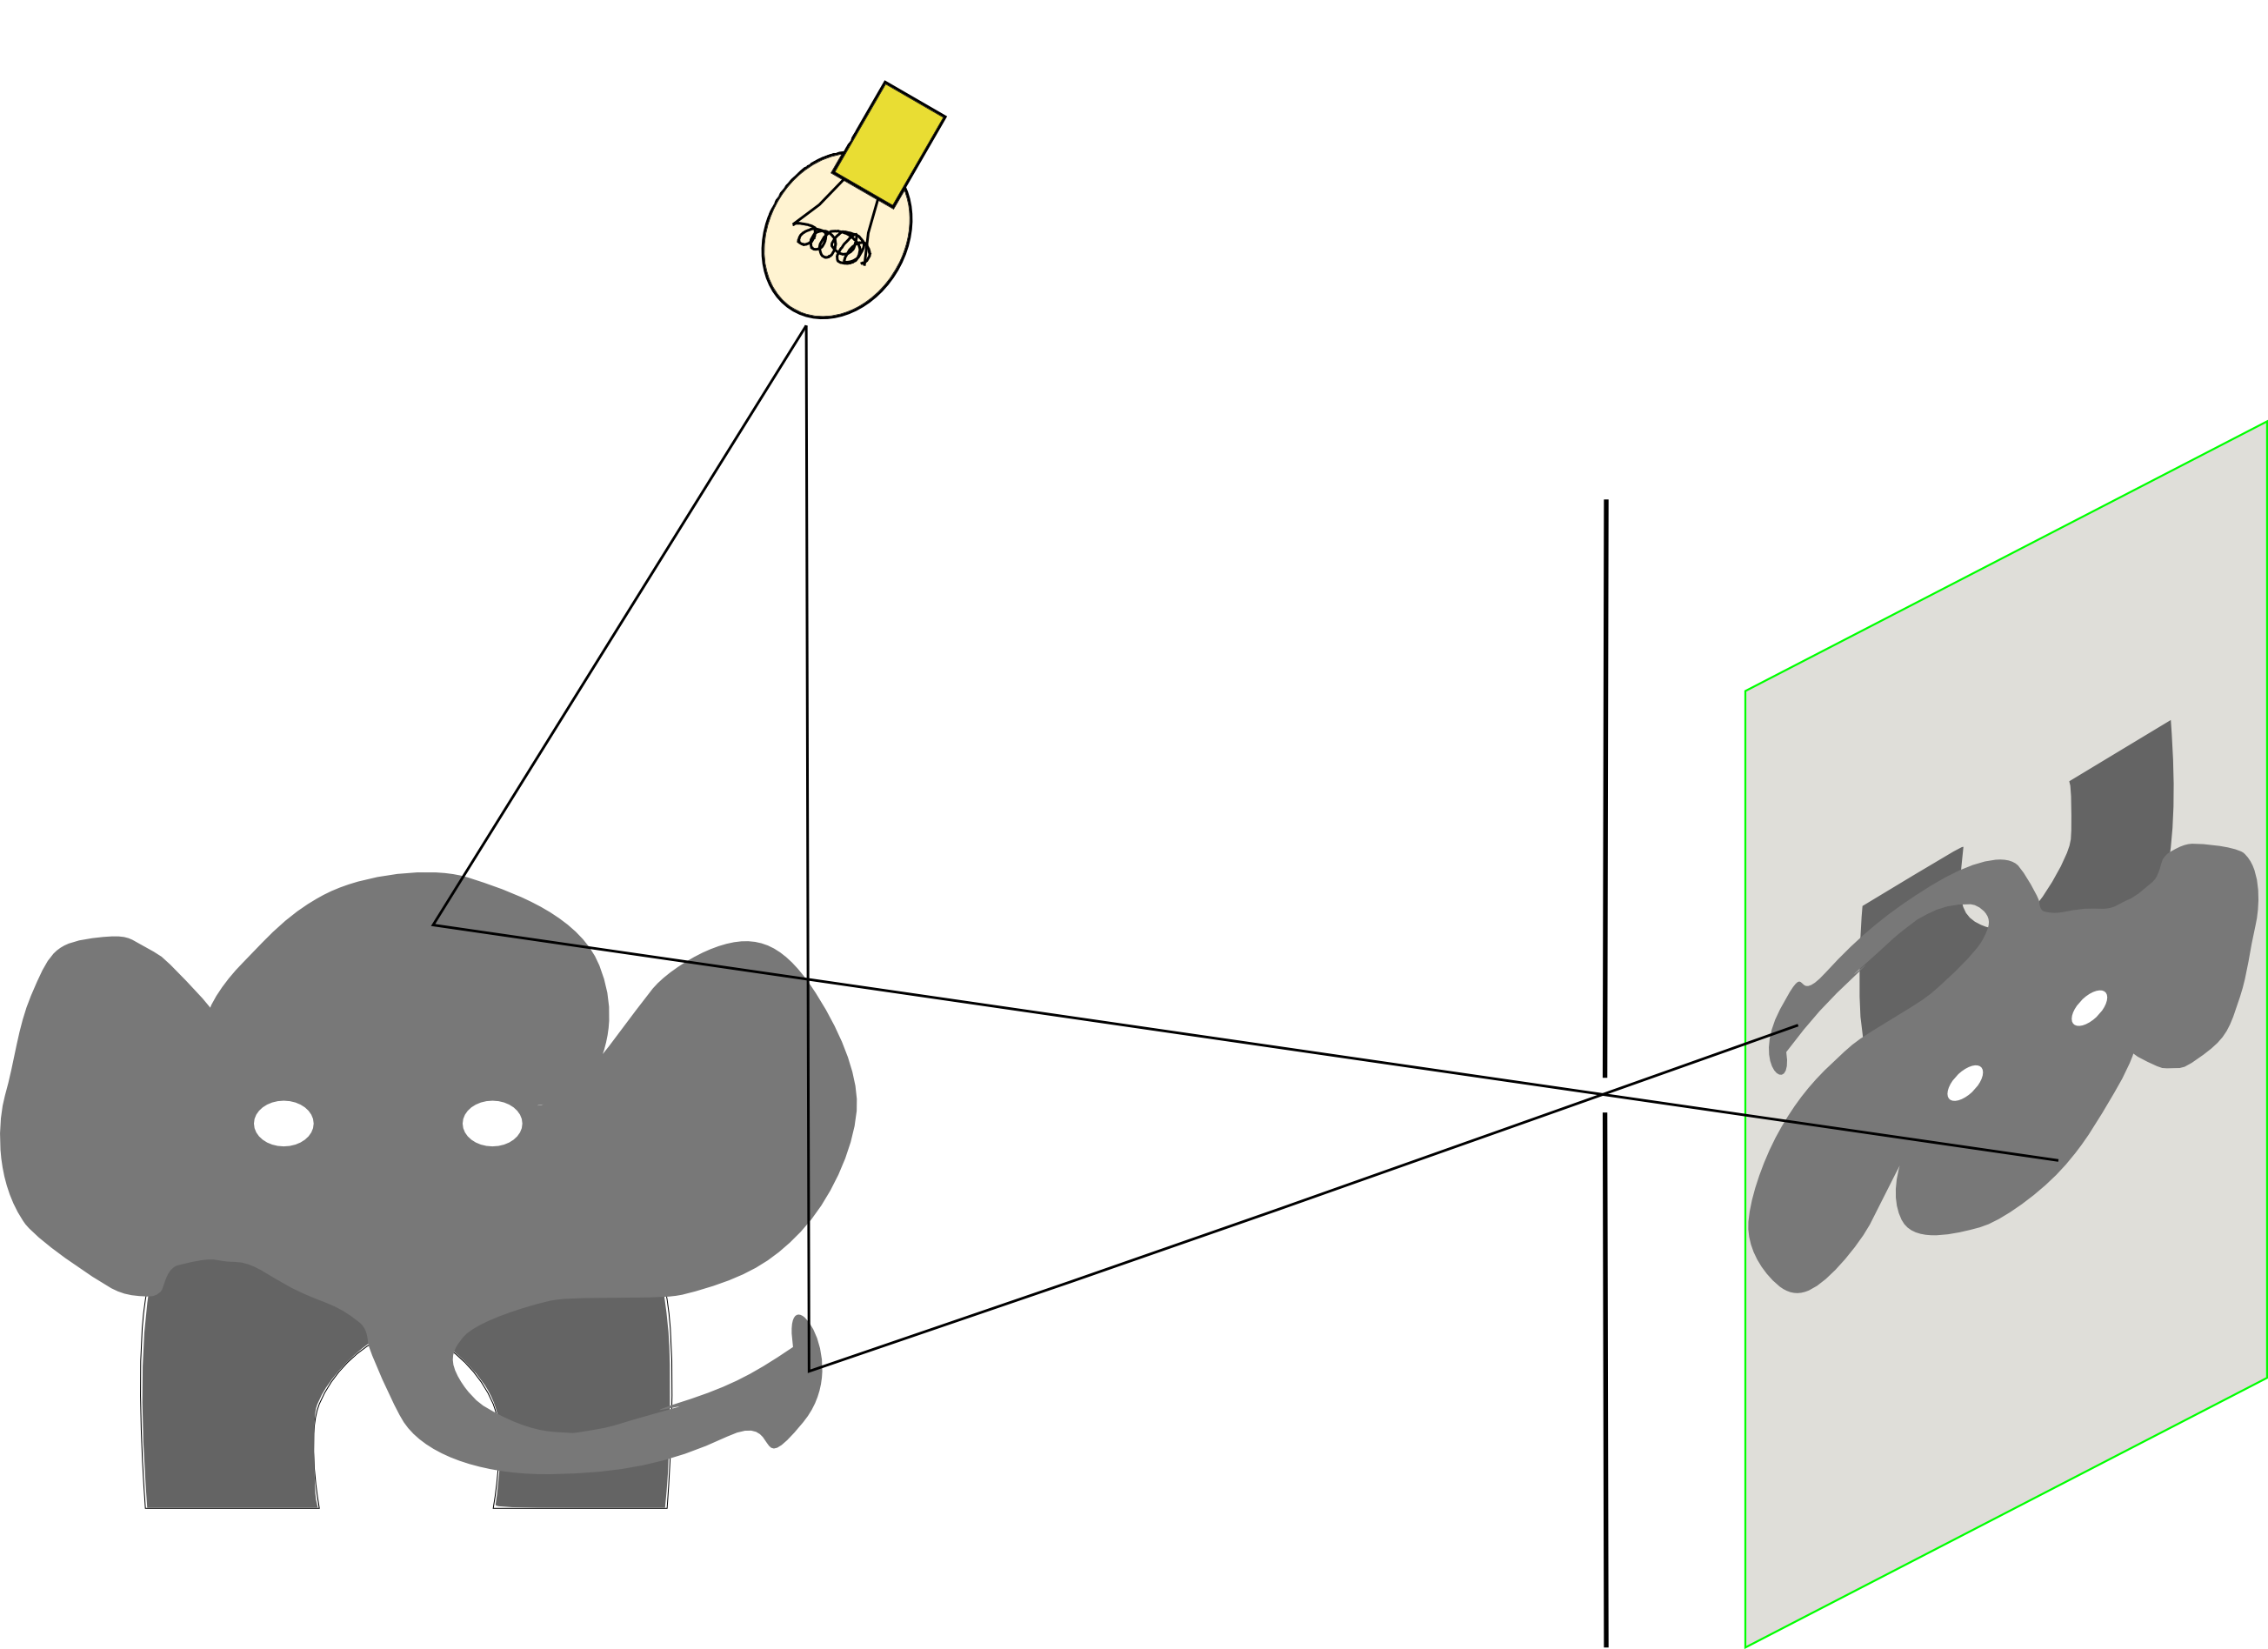
\includegraphics[width=0.65\textwidth]{FIGURES/oliphantpinhole}
%  \end{center}
%  Filtering the rays via a pinhole: get an (inverted) image. Principle
%  of the \myemph{Camera Obscura} (dark room).
% \end{frame}

% \section{A bit of History}


% ----------------------------------------------------
\begin{frame}
  \frametitle{Camera Obscura}
  \begin{center}
    \begin{tabular}[h]{cc}
       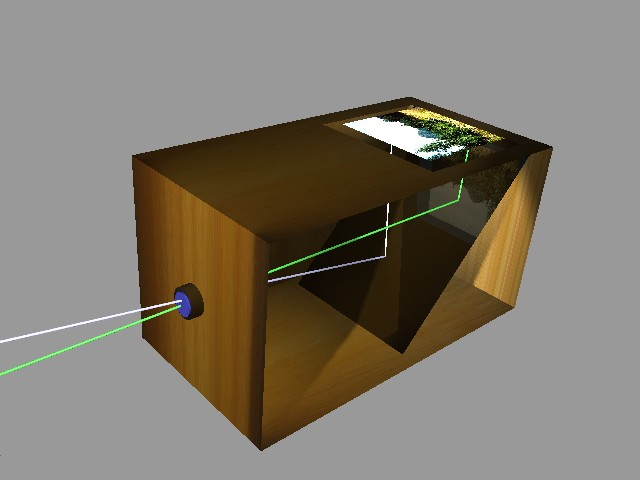
\includegraphics[width=0.4\textwidth]{IMAGES/WMCamera_obscura_box} &
       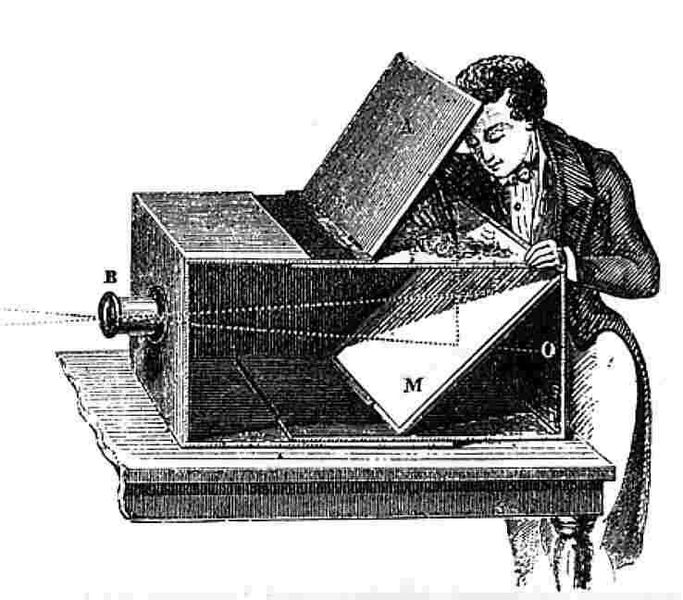
\includegraphics[width=0.4\textwidth]{IMAGES/WMCameraObscura18thCentury}\\
       Principle of Camera Obscura & 18th Century Camera Obscura
     \end{tabular}
   \end{center}
   \begin{itemize}
   \item Known from old chines writings
   \item Mentioned by Aristotle
   \item Plaque with photosensitive material: Photographic camera!
   \end{itemize}
 \end{frame}


% ----------------------------------------------------
 \begin{frame}
   \frametitle{The Very First Photography, 1826}
   \begin{center}
     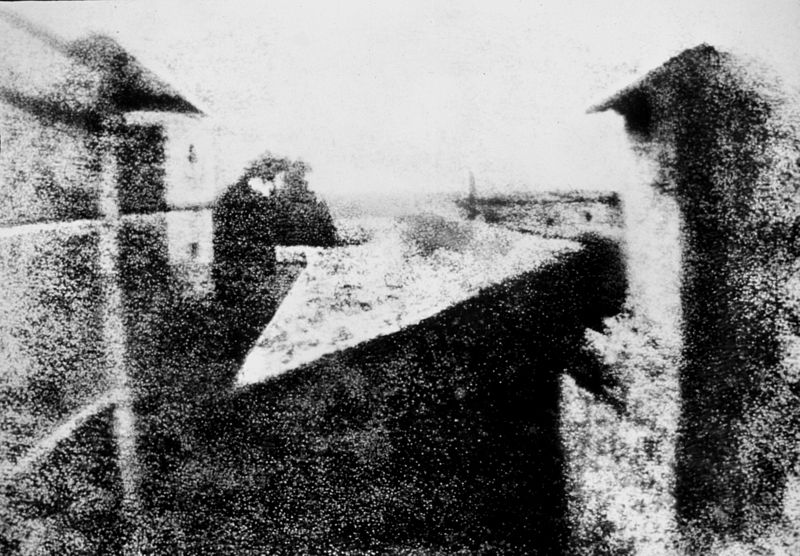
\includegraphics[width=0.8\textwidth]{IMAGES/WindowLegrasNiepce}
   \end{center}
   J.N. Ni�pce, View from the window at Le Gras,
   Saint Loup de Varennes, France -- Now at University of Texas at
   Austin.
 \end{frame}




% ----------------------------------------------------
 \begin{frame}
   \frametitle{The pin-hole camera}
   \begin{center}
     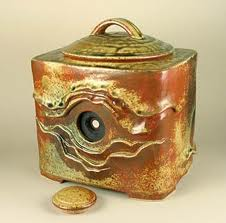
\includegraphics[width=0.4\textwidth]{IMAGES/pinholecamera.jpg}
     \hspace{2mm}
     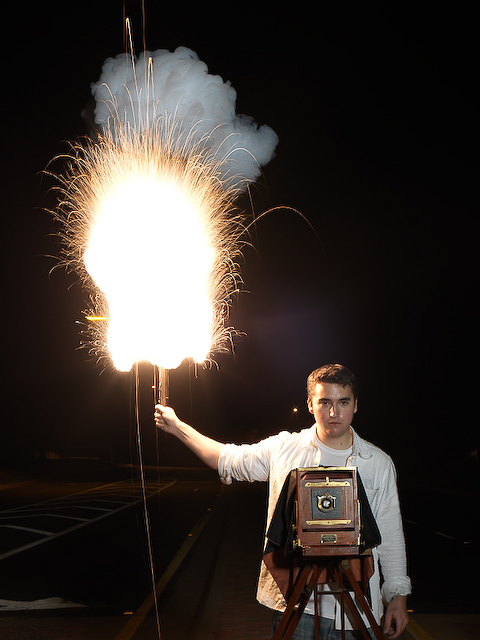
\includegraphics[width=0.4\textwidth]{IMAGES/magnesiumbomb.jpg}
   \end{center}
   Magnesium light was used to make light enough enter the pin-hole box.
 \end{frame}


% ----------------------------------------------------
% \begin{frame}
%    \begin{center}
%    \frametitle{The Pioneers}
%    \begin{tabular}[h]{ccc}
%      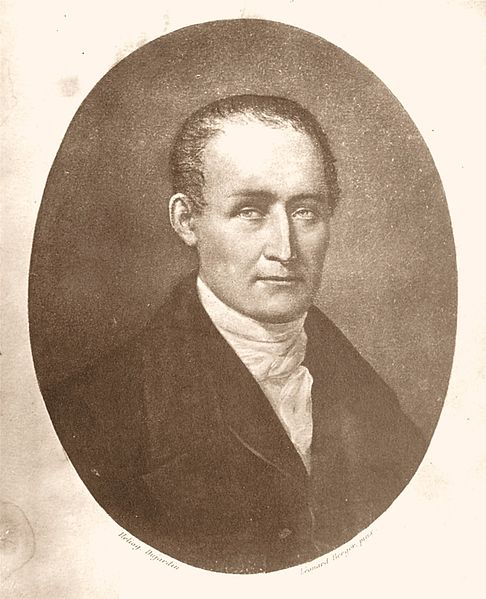
\includegraphics[width=0.3\textwidth]{IMAGES/JNNiepce} &
%      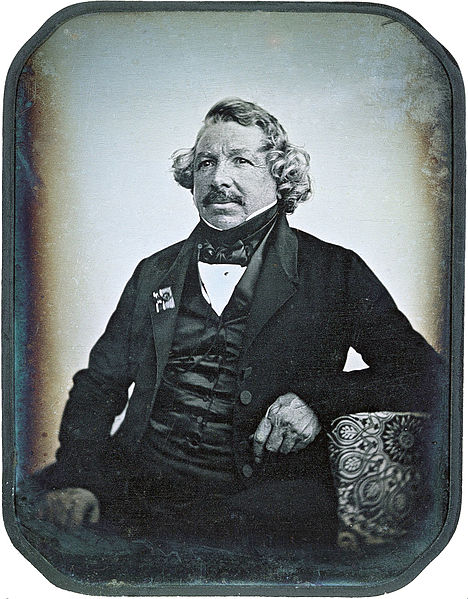
\includegraphics[width=0.3\textwidth]{IMAGES/LDaguerre} &
%      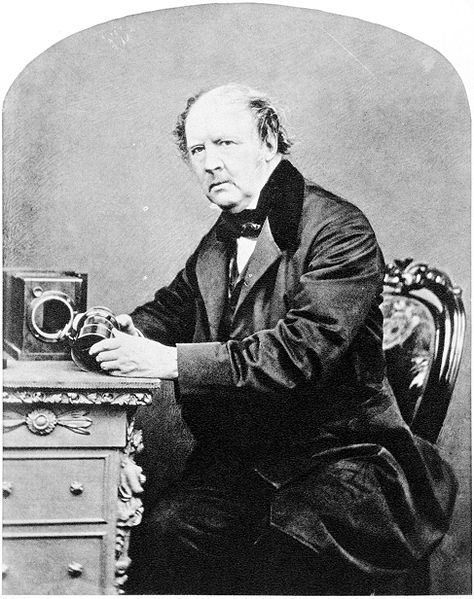
\includegraphics[width=0.3\textwidth]{IMAGES/HFTalbot} \\
%      J. Nicéphore Nièpce & Louis Daguerre & Henri F. Talbot
%    \end{tabular}
%  \end{center}
% \end{frame}


% ----------------------------------------------------
% \begin{frame}
%  \frametitle{Now...}
%  \begin{center}
%    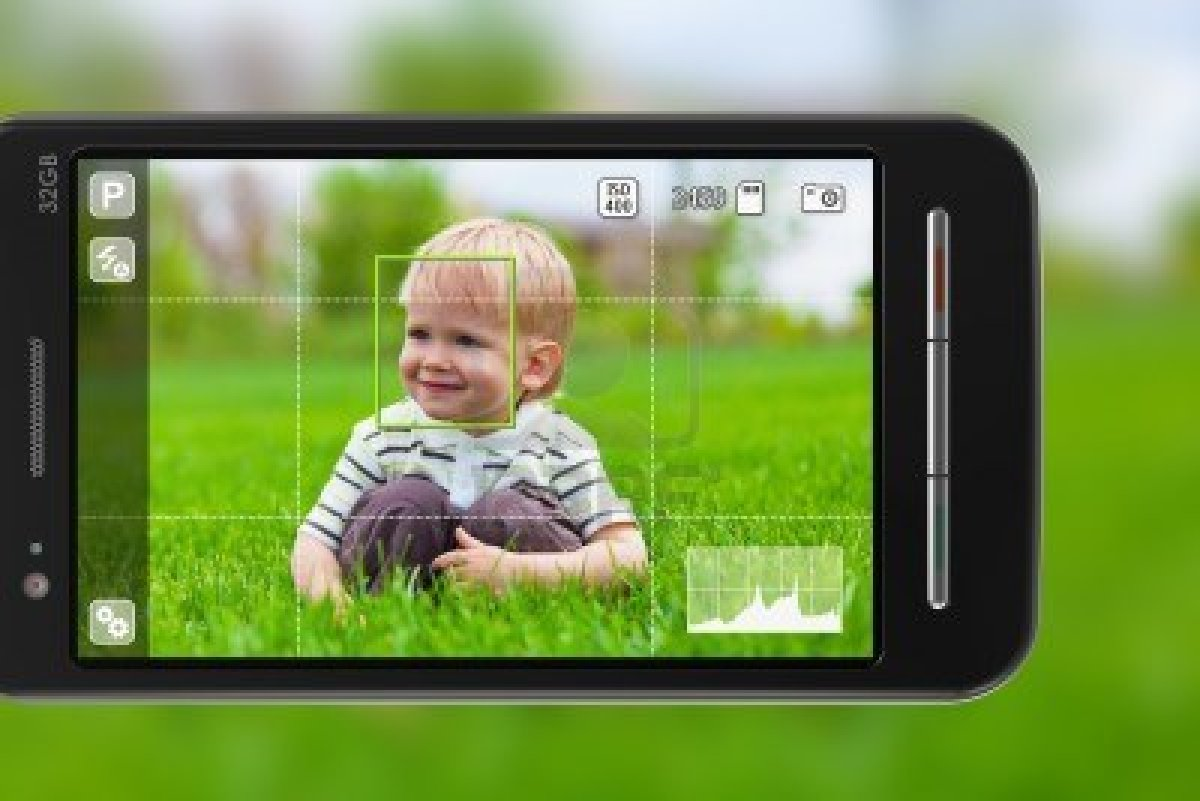
\includegraphics[width=0.8\textwidth]{IMAGES/smartphonecamera}
%  \end{center}
% \end{frame}



% \section{Projection}

% ----------------------------------------------------
 \begin{frame}
   \frametitle{The Pinhole Camera Model}
   \begin{center}
     \includegraphics[width=0.9\textwidth]{FIGURES/coproj}
   \end{center}
   \begin{itemize}
   \item $f$ is the focal length,
   \item $O$ is the camera center.
   \end{itemize}
 \end{frame}


% ----------------------------------------------------
% \begin{frame}
%   \frametitle{Projection is Tricky!}
%   \begin{center}
%     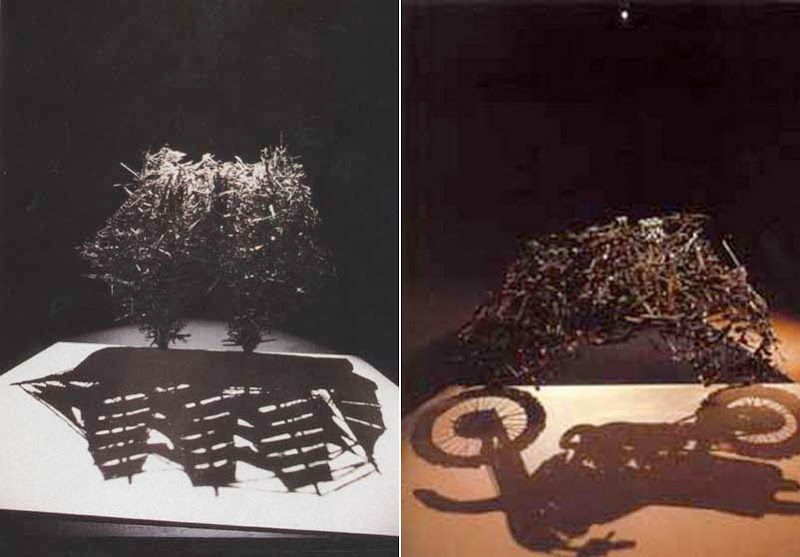
\includegraphics[width=0.9\textwidth]{IMAGES/shigeoFukuda}
%   \end{center}
%   Some illusions from Shigeo Fukuda. 
% \end{frame}



% ----------------------------------------------------
\begin{frame}
   \frametitle{Perspective Effects}
   Remember from first lecture
   \begin{center}
     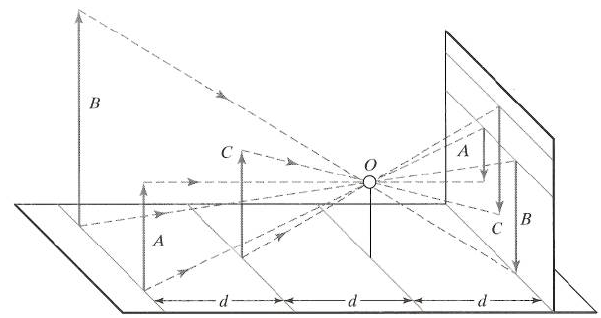
\includegraphics[width=0.9\textwidth]{FIGURES/fp131}
   \end{center}
   Far objects appear smaller that close ones.
 \end{frame}


% ----------------------------------------------------
 \begin{frame}
   \frametitle{Perspective Effects}
   Remember from first lecture again
   \begin{center}
     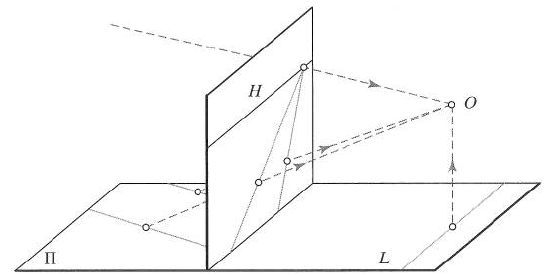
\includegraphics[width=0.9\textwidth]{FIGURES/fp132}
   \end{center}
   Images of parallel lines intersect at the horizon (virtual image plane).
 \end{frame}



% ----------------------------------------------------
% \begin{frame}
%  \frametitle{Stereo disparity}
%  \begin{center}
%    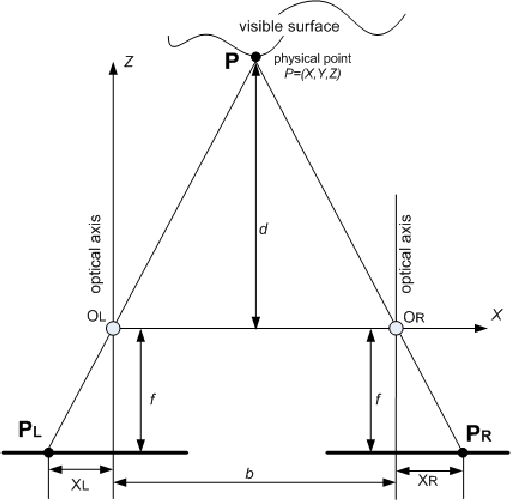
\includegraphics[width=0.9\textwidth]{MyImages/Stereo.png}
%   \end{center}
%  \begin{itemize}
%   \item Let the projection of $P$ on the baseline $O_L O_R$ be divided
%    in distances $A$ and $B$ and notice the two pairs of similar
%   triangles.
%  \item We have that $Z/A = f/x_L$ and that $Z/B = f/(-x_R)$.  Then
%    $$
%     b = A + B = Z \frac{x_L}{f} + Z \frac{-x_R}{f} = 
%    \frac{Z}{f} (x_L - x_R) = \frac{Z}{f}d
%    $$
%    where $d$ is the \myemph{disparity}.  Rewriting:
%   $$
%     Z = \frac{bf}{d}
%    $$
%   \end{itemize}
% \end{frame}


% ----------------------------------------------------
\begin{frame}
   \frametitle{Projection Equations}
   \begin{center}
    % 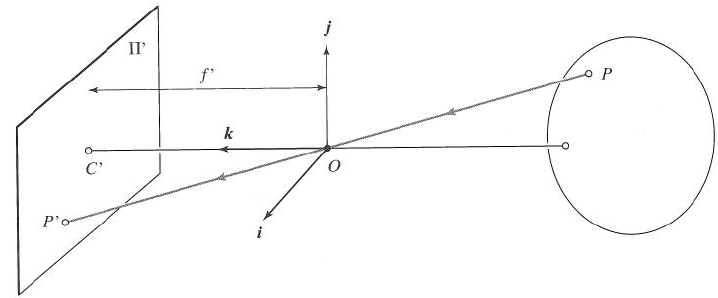
\includegraphics[width=0.9\textwidth]{FIGURES/fp14}
     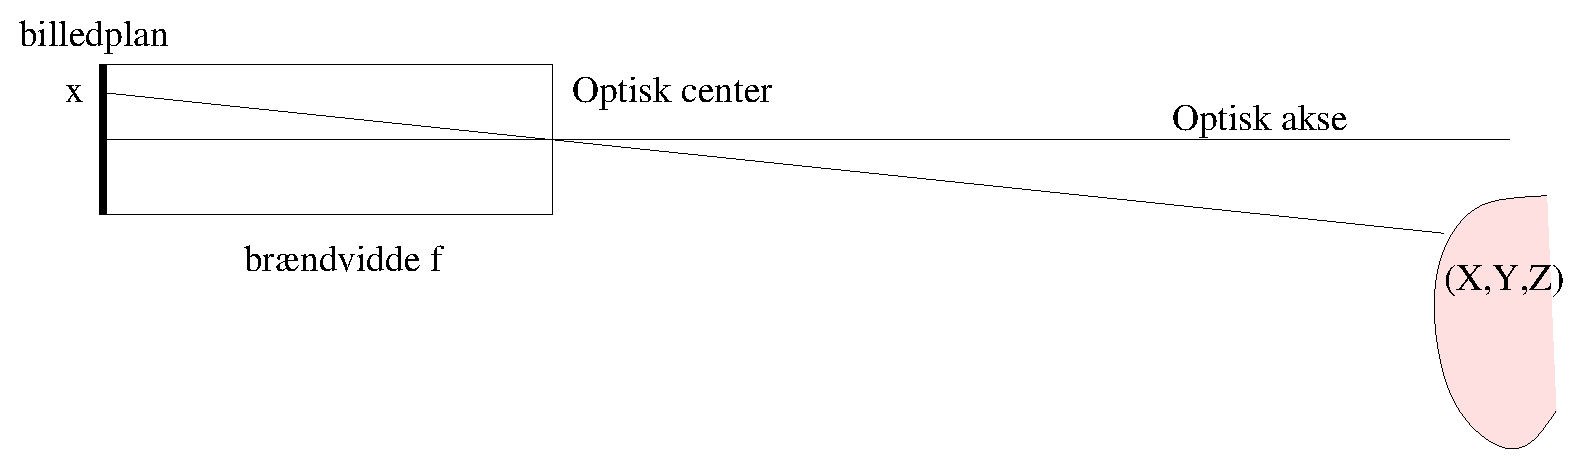
\includegraphics[width=0.9\textwidth]{FIGURES/pinholemodel.eps}
   \end{center}
   \begin{itemize}
     \item  Project $P (X,Y,Z)$ onto $ (x,y,-f)$.  Remember: similar triangles:
     $$
      x = f\frac{X}{Z},\quad y = f\frac{Y}{Z}
      $$
    \item To get non-negative pixel indexes:
     $$
      x \;=\; f\frac{X}{Z} \;+\; c_x ,\quad y \;=\; f\frac{Y}{Z} \;+\; c_y
      $$
      where $(c_x, c_y)$ is called {\color{red}{the principal point}}.
   \end{itemize}
 \end{frame}


% ----------------------------------------------------
 \begin{frame}
   \frametitle{Lost in projection}
     \begin{center}
     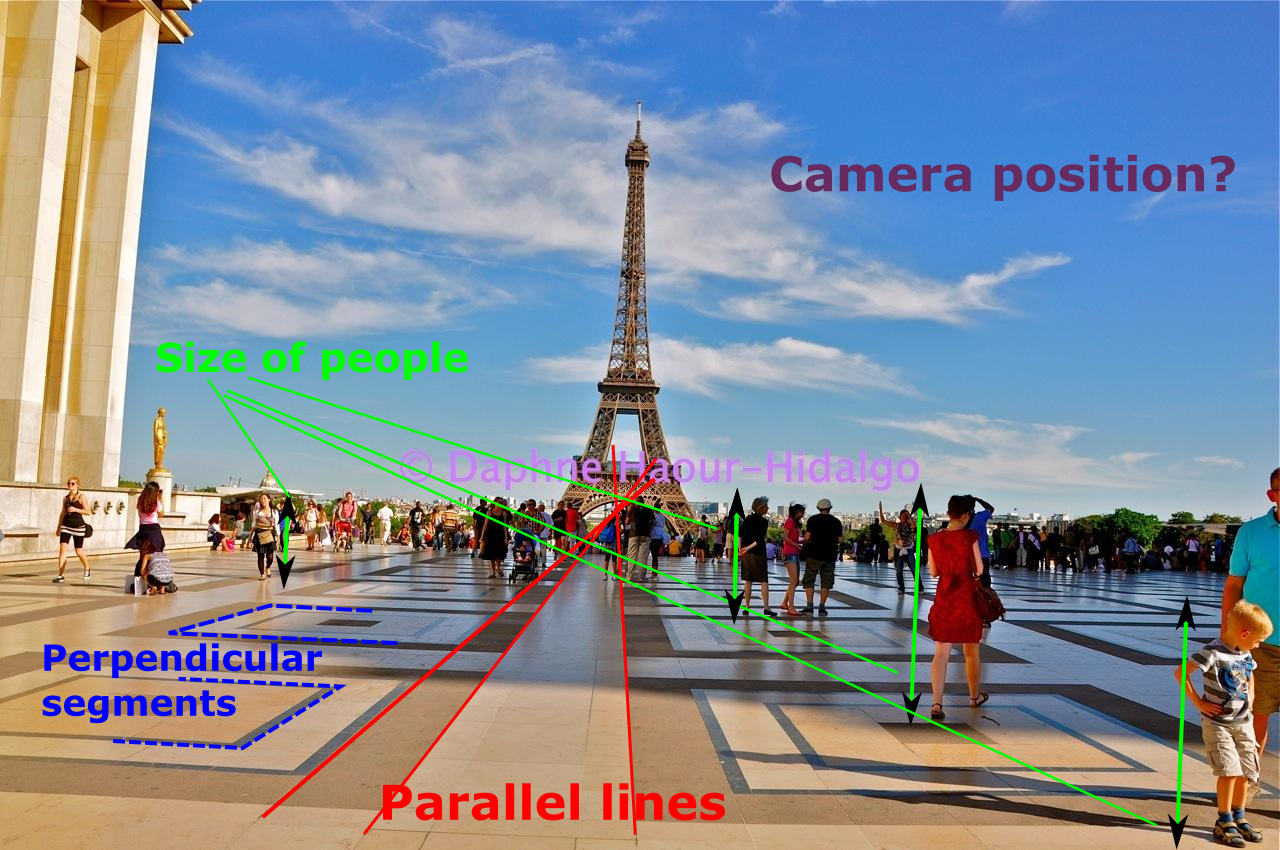
\includegraphics[width=0.8\textwidth]{IMAGES/trocadero_annotations}
   \end{center}
   Depth, Angles, size, parallelism.
 \end{frame}


% ----------------------------------------------------
 \begin{frame}
   \frametitle{Preserved by projection}
     \begin{center}
     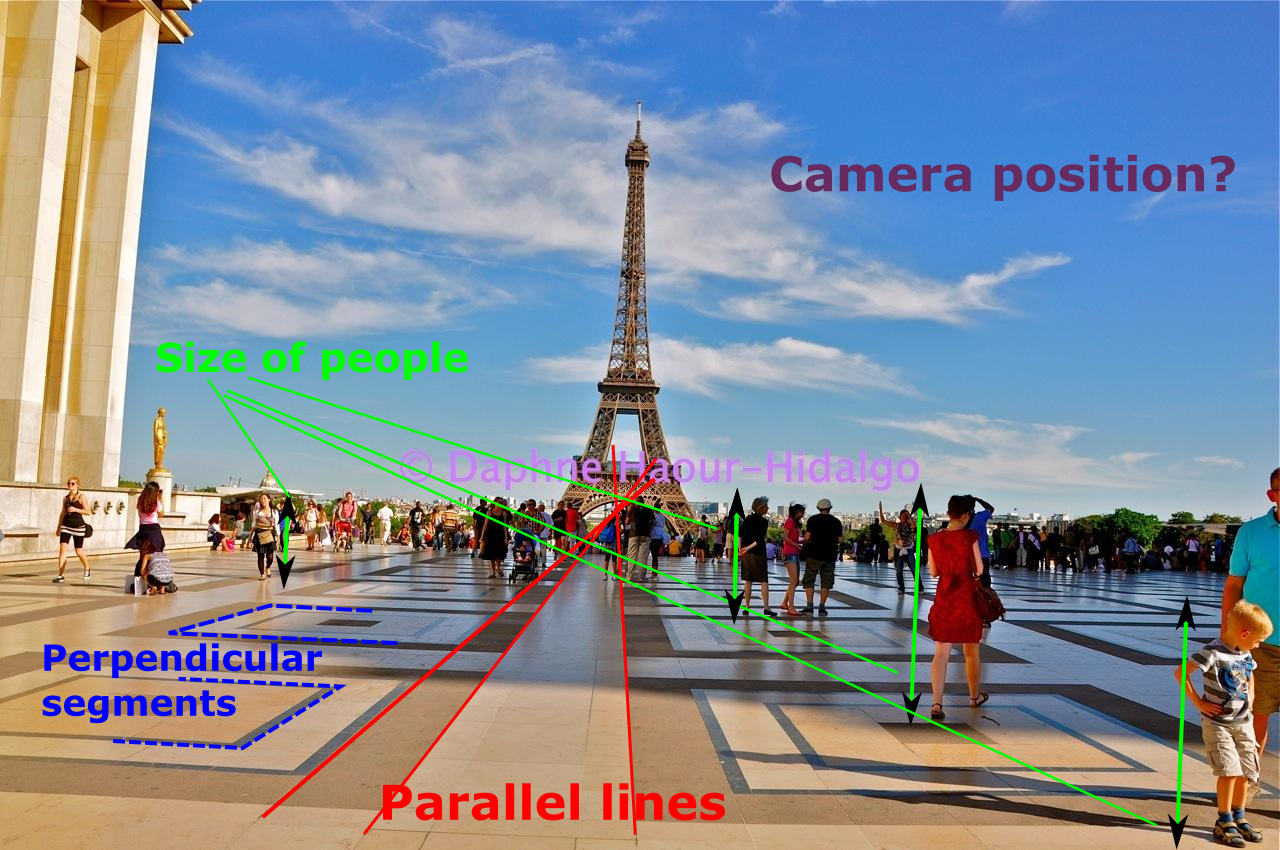
\includegraphics[width=0.8\textwidth]{IMAGES/trocadero_annotations}
   \end{center}
   Straight lines, connectivity, neighborhood.
 \end{frame}


% ----------------------------------------------------
 \begin{frame}
  \frametitle{Vanishing Points}
     \begin{center}
     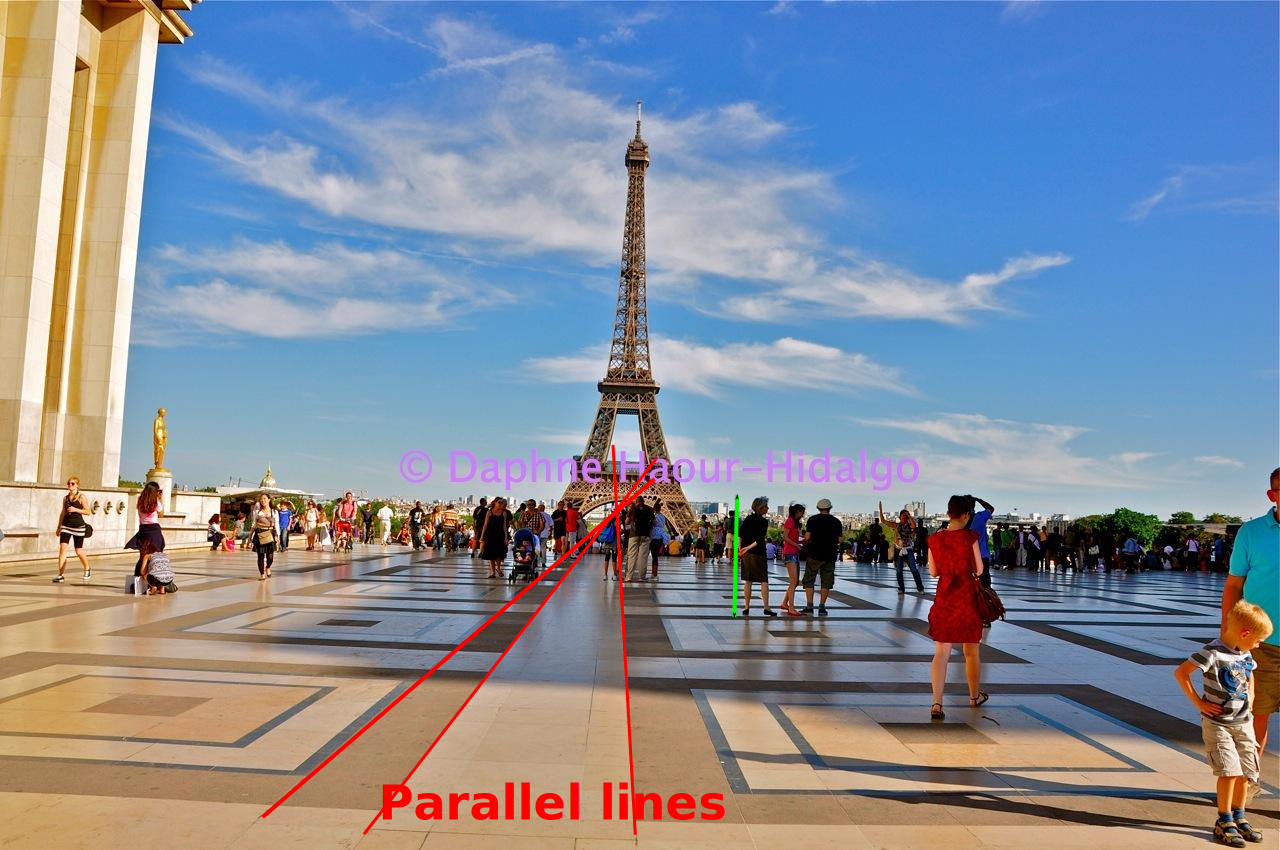
\includegraphics[width=0.8\textwidth]{IMAGES/trocaderolines}
  \end{center}
   Projections of parallel lines intersect at common points.
 \end{frame}



% ----------------------------------------------------
 \begin{frame}
 \frametitle{Vanishing line}
   \begin{center}
     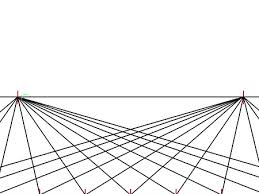
\includegraphics[width=0.4\textwidth]{IMAGES/vanishingline2.jpg}
     \hspace{2mm}
     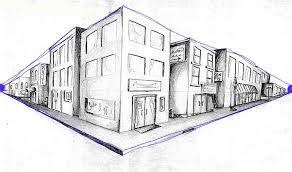
\includegraphics[width=0.4\textwidth]{IMAGES/vanishingline1.jpg}
   \end{center}
 \end{frame}


% ----------------------------------------------------
% \begin{frame}
%   \frametitle{Exercise}
% \begin{enumerate}
%   \item  {\color{red}{How many vanishing points can there be in an
%         image ?}} \\[3mm] 
%        \pause    
%        As many as there are planar sufaces with parallel linear
%        texture \\[4mm]
%   \item {\color{red}{Can we compute the vanishing line of a planar
%         surface from images of 1, 2 or, 3 different sets of parallel
%         lines on the surface?}} \\[3mm]
%         \pause
%         Yes, we need 2 sets of parallel lines.  This gives 2 VPs and
%         the VL connecting them. \\[4mm]
%    \item {\color{red}{May we compute 3D surface orientation (the
%          surface normal)  from a vanishing line?}} \\[3mm]
%       \pause
%       Yes, if we know the focal length $f$ of the camera.  If the
%       VL-equation is $Ax + By + C = 0$ then the 3D surface normal
%       will be $(-\frac{f A}{C},  -\frac{f B}{C}, -1)$.
% \end{enumerate}
% \end{frame}



% ----------------------------------------------------
\begin{frame}
   \frametitle{Vanishing line}
   \begin{center}
     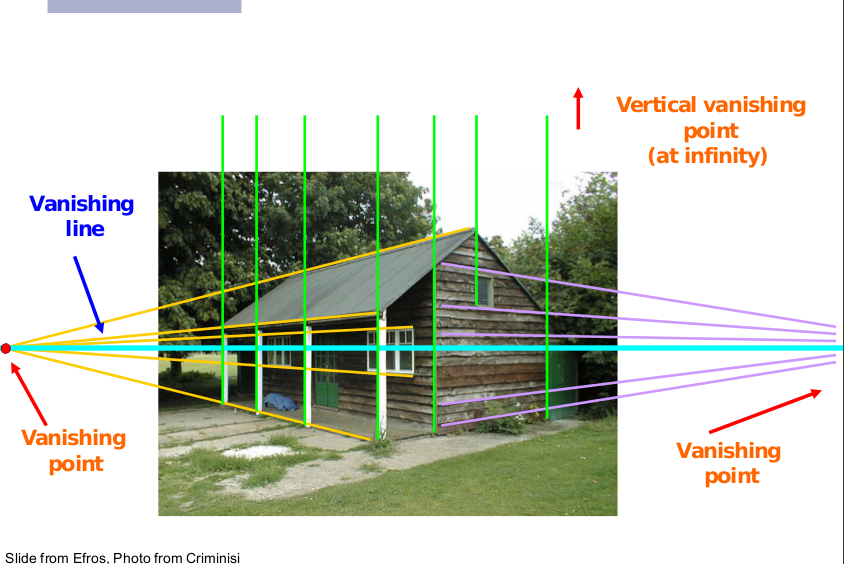
\includegraphics[width=0.8\textwidth]{FIGURES/vanishingline}
   \end{center}
 \end{frame}



% ----------------------------------------------------
 \begin{frame}
   \frametitle{Shape (VP's) from texture}
     \begin{center}
      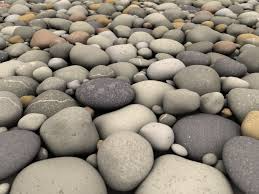
\includegraphics[width=0.65\textwidth]{IMAGES/stonetexture.png}
     \end{center}

 If we can measure a texture density, then we may estimate the
 directions of minimal and maximal density change. Theses points at the
 VPs.
  thus giving the VL and the 3D surface normal.
 \end{frame}


% ----------------------------------------------------
% \begin{frame}
% \frametitle{Shape from texture}
% The 3D shape (surface normal) of a uniformly textured scene surface
% may be estimated from the projected texture.
%
% \begin{center}
%   \includegraphics[width=0.75\textwidth]{Images/texturedhills.jpg}
% \end{center}
% 
% Sign up for ATIA if you want to learn more about texture.
% 
% \end{frame}


% ----------------------------------------------------
\begin{frame}
  \frametitle{Homogeneous coordinates 1D}
 {\small
  \begin{itemize}
  \item In 1D coordinate is just 1 number. 
    \begin{center}
      
\includegraphics[width=0.75\textwidth]{FIGURES/1dcoords}
    \end{center}
  \item 1D coordinate to 1D Homogeneous coordinates: 
    $$x\sim
    \begin{bmatrix}
      x\\1
   \end{bmatrix}
    $$
  \item 1D homogeneous coordinate to 1 D coordinate
    $$
     \begin{bmatrix}
      x\\w
    \end{bmatrix}\sim x/w 
    $$
  \item What can we do with that? we can ``tame'' infinity!
  \item A point with homogeneous coordinate $[x,0]^T$ has ``normal'' coordinate $x/0 = \infty$
    as if we took homogeneous coordinate $[\infty,1]^T$
    \begin{center}
      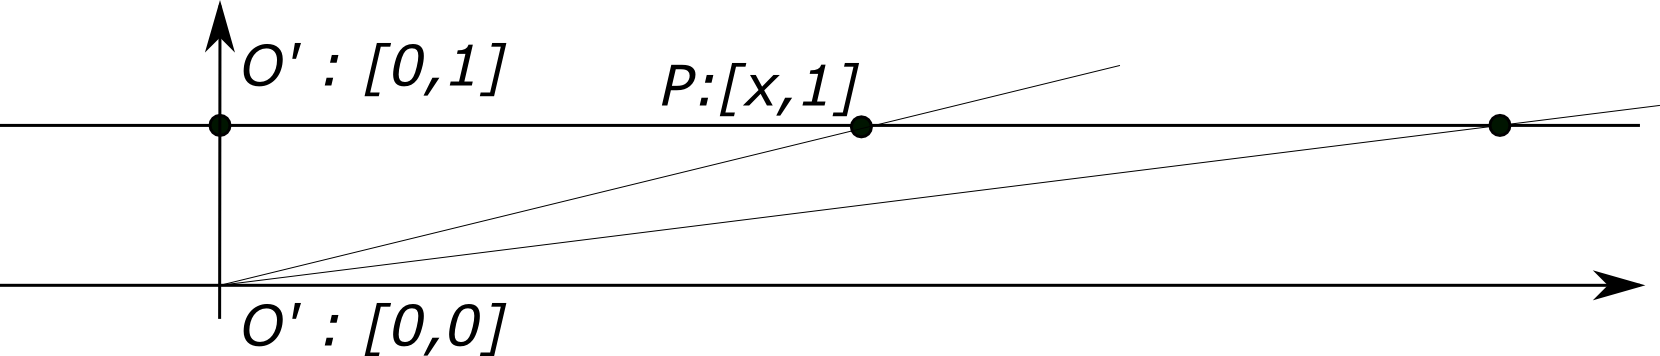
\includegraphics[width=0.75\textwidth]{FIGURES/1dcoordshomog}
    \end{center}
  \end{itemize}
  }
\end{frame}


% ----------------------------------------------------
\begin{frame}
  \frametitle{Homogeneous coordinates, 2D}
  ``Natural Coordinates'' for projective geometry
  \begin{itemize}
  \item From 2D point coordinate to 2D Homogeneous coordinate
    $$
    (x,y)\Implies
    \begin{bmatrix}
      x\\y\\1
    \end{bmatrix}
    $$
  \item From 2D homogeneous coordinates to 2D coordinates
    $$   
    \begin{bmatrix}
      x\\y\\w
    \end{bmatrix}
    \Implies 
    (x/w, y/w)
    $$
%   % \item Exercise: Let $P$ have coordinates $(x,y,1)$ and let
%   %   $Q(x',y',w)$ be a point on the line through $O (0,0,0)$ and $P$.  Compute $x'$ and $y'$.
%   %   Considering $[x',y',w]$ as homogeneous 2D coordinates, what are
%   %   the corresponding 2D coordinates?
  \end{itemize}
\end{frame}


% ----------------------------------------------------
\begin{frame}
  \frametitle{Homogeneous coordinates, 3D}
  \begin{itemize}
  \item From 3D point coordinate to 3D Homogeneous coordinate
    $$
    (x,y,z)\Implies
    \begin{bmatrix}
      x\\y\\z\\1
    \end{bmatrix}
    $$
  \item From 3D homogeneous coordinates to 3D coordinates
    $$   
    \begin{bmatrix}
      x\\y\\z\\w
    \end{bmatrix}
    \Implies 
    (x/w, y/w, z/w)
    $$
  \end{itemize}
\end{frame}


% ----------------------------------------------------
\begin{frame}
  \frametitle{Homogeneous coordinates}
  \begin{center}
    
\includegraphics[width=0.7\textwidth]{FIGURES/projcoords1}
  \end{center}
  Homogeneous coordinates in 2D correspond to points in plane $z=1$
  but also to lines through the origin and this point.
\end{frame}


% ----------------------------------------------------
\begin{frame}
  \frametitle{Cameras and homogeneous coordinates}
  \begin{itemize}
  \item Projection to image plane in standard coordinates:
    $$
    P: (x,y,z)\mapsto P': (f\frac{x}{z}, f\frac{y}{z})
    $$
  \item How does the mapping look like in homogeneous coordinates:
    $$
    P:
    \begin{bmatrix}
      x\\y\\z\\1
    \end{bmatrix}
    \mapsto P': 
    \begin{bmatrix}
      fx\\fy\\z
    \end{bmatrix}
    $$
  \item Matrix notation
    $$
     \begin{bmatrix}
      fx\\fy\\z
    \end{bmatrix}
    = \udesc{K}{
    \begin{pmatrix}
      f & 0 & 0 & 0\\
      0 & f & 0 & 0\\
      0 & 0 & 1 & 0
    \end{pmatrix}}
    \begin{bmatrix}
      x\\y\\z\\1
    \end{bmatrix}
    $$
    \item $K$ is (a simple version of) the \myemph{Camera Calibration
        Matrix} and contains the intrinsic calibration parameters
      (here $f$).
  \end{itemize}
\end{frame}


% ----------------------------------------------------
\begin{frame}
  \frametitle{World, Camera and Image Coordinates}
  In the previous slides we were not precise on the many coordinate
  systems are implicitly used:\\[3mm] 
  \begin{itemize}
  \item 3D World Coordinates: Coordinate system of the 3D world. \\[3mm]
  \item Camera Coordinates: 3D coordinate system attached to the camera. \\[3mm]
  \item Image Coordinates: 2D Coordinate system attached to the image plane. \\[3mm]
  \item The coordinate system for the sampled and digitised image \\[3mm]
  \end{itemize}
\end{frame}


% ----------------------------------------------------
% \begin{frame}
%   \frametitle{Assumptions Behind the Simple Model}
%   \begin{center}
%     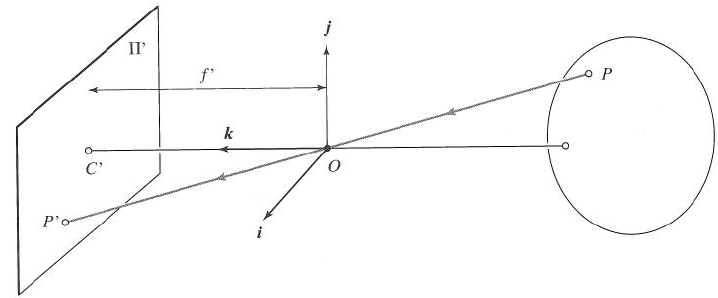
\includegraphics[width=0.8\textwidth]{FIGURES/fp14}
%   \end{center}
%   \begin{itemize}
%     \item The camera center $0$ is the same as the image coordinates origin,
%     \item The axes (base vectors) $\bi$, $\bj$ and $\bk$ are common
%       for the camera and the image coordinate systems
%     \item Pixels are squared and perfectly aligned with the camera coordinates
%     \item $C'$,  the projection of the camera center $O$ is called the
%       principal point and have coordinates given by the position of
%       the imaging device and the sampling used.
%   \end{itemize}
% \end{frame}


% ----------------------------------------------------
\begin{frame}
  \frametitle{Intrinsic vs Extrinsic Camera Parameters}
  Intrinsic parameters refer to {\color{blue}{internal parameters}}:
  \begin{itemize}
  \item The principal point: 2 parameters
  \item Scale factors (or sampling frequencies)  for the pixels sizes
    in both x and y directions: 2 parameters, multiplied by the focal
    length, resulting in {\color{blue}{the effective focal length}} 
    $(f_x, f_y) = f \cdot (s_x, s_y)$.
  \item Skewness of pixels: 1 parameter. (Often assumed zero)
  \end{itemize}
  {\color{blue}{Extrinsic Camera parameters}}:
  \begin{itemize}
  \item Position of the camera coordinate system in the world coordinates system:
    translation: 3 parameters,
  \item Orientation of the camera coordinate system in the world coordinates system:
    rotation: 3 parameters.
  \end{itemize}
\end{frame}


% ----------------------------------------------------
\begin{frame}
  \frametitle{Oriented and Translated Camera}
  \begin{center}
    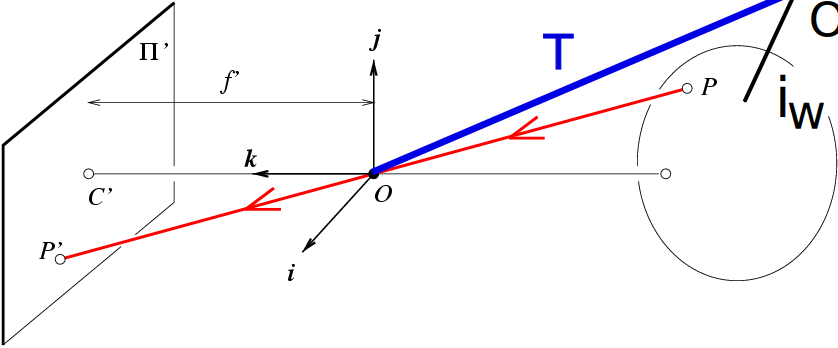
\includegraphics[width=0.9\textwidth]{FIGURES/orientedtranslatedcam1}
  \end{center}
\end{frame}


% ----------------------------------------------------
\begin{frame}
  \frametitle{Translating Coordinate System}
  \begin{center}
   
\includegraphics[width=0.5\textwidth]{FIGURES/translation3D} 
  \end{center}
%  Assume $O'$ at coordinates $(x_{O'},y_{O'},z_{O'})$ in coordinate system
%  $(O,\bi,\bj,\bk)$ and $P$ has coordinates $(x,y,z)$ also in $(O,\bi,\bj,\bk)$.
%  What are its coordinates in $(O',\bi,\bj,\bk)$?
% \end{frame}
%
%
% ----------------------------------------------------
% \begin{frame}  
  \begin{itemize}
%   \item Let $(x',y',z')$ its coordinates in $(O,\bi,\bj,\bk)$.
%   \item Write $\overrightarrow{O'P}$ = $\overrightarrow{OP} - \overrightarrow{OO'}$
%   \item Develop:
     \item Subtract the translation vector:
     $$
     \begin{pmatrix}
       x'\\y'\\z'
     \end{pmatrix}
     = 
     \begin{pmatrix}
       x\\y\\z
     \end{pmatrix}
     -
     \begin{pmatrix}
       x_{O'}\\y_{O'}\\z_{O'}
     \end{pmatrix}
     =
     \begin{pmatrix}
       x-x_{O'}\\y-y_{O'}\\z-z_{O'}
     \end{pmatrix}
     $$
   \item Transformation in homogeneous coordinates:
     $$
     \begin{bmatrix}
       x'\\y'\\z'\\1
     \end{bmatrix}
     =
     \begin{pmatrix}
       1 & 0 & 0 & -x_{O'}\\
       0 & 1 & 0 & -y_{O'}\\
       0 & 0 & 1 & -z_{O'}\\
       0 & 0 & 0 & 1
     \end{pmatrix}
     \begin{bmatrix}
       x\\y\\z\\1
     \end{bmatrix}
     $$
   \end{itemize}
 \end{frame}


% ----------------------------------------------------
 \begin{frame}
   \frametitle{Rotating Coordinate System}
   \begin{columns}
     \column{0.5\textwidth}
     \begin{center}
       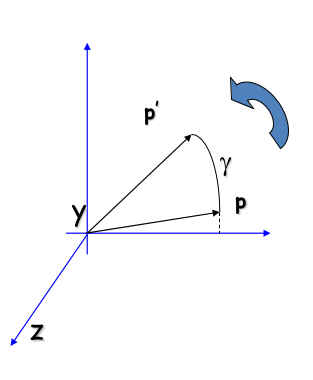
\includegraphics[width=\textwidth]{FIGURES/rotation3d}
     \end{center}
     \column{0.5\textwidth}
     Rotations along coordinate axes
     $$
     R_{x\alpha} = 
     \begin{pmatrix}
       1 & 0 & 0\\
       0 & \cos\alpha & -\sin\alpha\\
       0 & \sin\alpha & \cos\alpha
     \end{pmatrix}
     $$
     $$
     R_{y\beta} = 
     \begin{pmatrix}
       \cos\beta & 0 & -\sin\beta\\
       0 & 1 & 0\\
       \sin\beta & 0 & \cos\beta
     \end{pmatrix}
     $$
     $$ 
     R_{z\gamma} = 
     \begin{pmatrix}
       \cos\gamma & -\sin\gamma & 0\\
       \sin\gamma & \cos\gamma & 0\\
       0 & 0 & 1
     \end{pmatrix}
     $$
   \end{columns}~\\
   ~\\
   Can also be written in homogeneous coordinates
 \end{frame}
 

% ----------------------------------------------------
 \begin{frame}
   \frametitle{3D rotations}
To obtain a 3D rotation apply all 3 single-axis rotations:
{\small
\begin{eqnarray*}
     R &=&  R_{x\alpha}   R_{y\beta}  R_{z\gamma} \\[3mm]
        &=&
     \begin{pmatrix}
       1 & 0 & 0\\
       0 & \cos\alpha & -\sin\alpha\\
       0 & \sin\alpha & \cos\alpha
     \end{pmatrix}
     \;\;
     \begin{pmatrix}
       \cos\beta & 0 & -\sin\beta\\
       0 & 1 & 0\\
       \sin\beta & 0 & \cos\beta
     \end{pmatrix}
     \;\;
     \begin{pmatrix}
       \cos\gamma & -\sin\gamma & 0\\
       \sin\gamma & \cos\gamma & 0\\
       0 & 0 & 1
     \end{pmatrix} 
\end{eqnarray*}
}
\vspace{3mm}

Please notice that the order of the 3 rotation matrices do
matter. However, no matter which order $(\alpha, \beta, \gamma)$ may
be found such that the resulting 3D rotation is correct.
\end{frame}
 

% ----------------------------------------------------
 \begin{frame}
   \frametitle{Camera Matrix}
   \begin{itemize}
%   \item Combine world vs camera coordinates with
   \item Camera calibration matrix, now extended with
     Image plane transformation (axis scalings, shear, translation)
     $$
     {\bf C} = {\bf K} \left[{\bf  R}\,\, {\bf t}\right]
     $$
   \item ${\bf K}$$3\times 3$ matrix encoding the homogeneous transformations
     inside the camera. ${\bf K}$ specifies the \myemph{Intrinsic parameters}.
   \item $\left[{\bf R}\,\, {\bf t}\right]$ Concatenation of world
     coordinates rotation and origin translation to align camera and
     world coordinates.
   \end{itemize}
   $$
   \begin{bmatrix}
     x \\y \\1
   \end{bmatrix}
   =   \begin{bmatrix}
     w x \\w y \\w 
   \end{bmatrix}
   =\udesc{{\bf K}}{
     \begin{pmatrix}
       f_x & s & u_0\\
       0 & f_y & v_0\\
       0 & 0 & 1
     \end{pmatrix}}
   \udesc{\left[{\bf R}\,\, {\bf t}\right]}{
     \begin{pmatrix}
       r_{11} & r_{12} & r_{13} & t_x\\
       r_{21} & r_{22} & r_{23} & t_y\\
       r_{31} & r_{32} & r_{33} & t_z\\
     \end{pmatrix}}
   \begin{pmatrix}
     X\\Y\\Z\\1
   \end{pmatrix}
   $$
 \end{frame}
 


%----------------------------------------------
\begin{frame}
\frametitle{Exercise}
\begin{itemize}
   \item {\color{red}{How many independent parameters are there to
        estimate in a camera calibration ?}} \\[3mm]
    \pause
      11: 5 intrinsic and 6 extrinsic (sometimes simplified to 3+6) \\[4mm]
   \item {\color{red}{May all calibration parameters be found using
         Linear algebra ?}} \\[3mm] 
    \pause
     No, they don't appear in a linear combinations. Some are
     multiplied together. 
 \end{itemize}
 \end{frame}
 


%-------------------------------------------------------------------
\begin{frame}
  \begin{center}
    {\color{blue}{\Huge QUESTIONS ?}}
  \end{center}
 \end{frame}



 


% ----------------------------------------------------
 \begin{frame}
   \frametitle{Geometric Calibration}
   \begin{itemize}
     \item Computing the camera matrix is called geometric calibration.
     \item Extrinsic parameters: (R,t): 
       Usually easy, but requires metric knowledge on scene features.
     \item Intrinsic parameters: (${\bf K}$): 
       Some parameters ($f$) are easy  and
       some ($(u_0, v_0)$) are difficult to estimate correctly.
   \end{itemize}
   \begin{columns}
     \column{0.5\textwidth}
     \begin{center}
       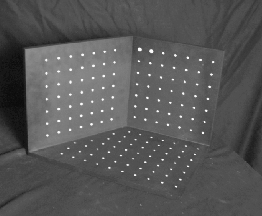
\includegraphics[width=0.8\textwidth]{IMAGES/calibrationobject}
     \end{center}
     \column{0.5\textwidth}
     \begin{itemize}
     \item Use an object with known geometry
     \item Use vanishing points / lines
     \item Use other cues...
     \end{itemize}
   \end{columns}
 \end{frame}


% Camera calibration ??? 

%----------------------------------------------
\begin{frame}
\frametitle{Repetition: The camera matrix}
Please recall the definition of the camera matrix:
\begin{displaymath}
      M =  K \left[ R \,\, {\bf t}\right]
\end{displaymath}
and the projection written out:
\begin{displaymath}
   w
   \begin{bmatrix}
     x\\y\\1
   \end{bmatrix}
   = \udesc{{\bf M}}{
      \udesc{{\bf K}}{
     \begin{pmatrix}
       f_x & 0 & u_0\\
       0 & f_y & v_0\\
       0 & 0 & 1
     \end{pmatrix}}
   \udesc{\left[{\bf R}\,\, {\bf t}\right]}{
     \begin{pmatrix}
       r_{11} & r_{12} & r_{13} & t_x\\
       r_{21} & r_{22} & r_{23} & t_y\\
       r_{31} & r_{32} & r_{33} & t_z\\
     \end{pmatrix}}}
   \begin{pmatrix}
     X\\Y\\Z\\1
   \end{pmatrix}
\end{displaymath}
or
\begin{displaymath}
   w
   \begin{bmatrix}
     x\\y\\1
   \end{bmatrix}
   =
     \begin{pmatrix}
       {\bf m}^1 \\
       {\bf m}^2 \\
       {\bf m}^3 \\
     \end{pmatrix}
   \begin{pmatrix}
     X\\Y\\Z\\1
   \end{pmatrix}
   =
     \begin{pmatrix}
       {\bf m}^1 U \\
       {\bf m}^2 U \\
       {\bf m}^3 U \\
     \end{pmatrix}
\end{displaymath}
where ${\bf m}^i$ is the $i$'th row of the camera matrix. 
\end{frame}



%----------------------------------------------
\begin{frame}
\frametitle{Camera calibration}
In Camera calibration the task is to recover the 12 unknowns ${\bf m}_{ij}$
in the camera calibration matrix.  Converting the result before to
image coordinates we have: 
\begin{eqnarray*}
   x {\bf m}_3 U & = & {\bf m}_1 U \\
   y {\bf m}_3 U & = & {\bf m}_2 U 
\end{eqnarray*}

Let ${\bf m} = (m_{11}, \ldots , m_{14} , \ldots, m_{34})^{\top}$ be the
vector of the 12 unknowns.  Isolating these in the equations above
lead to: $A {\bf m} = 0$, where:

{\tiny
\begin{displaymath}
 A \;=\; \left [
    \begin{array}{cccccccccccc}
       X_1 & Y_1 & Z_1 & 1 & 0 & 0 & 0 & 0 & -x_1X_1 & -x_1Y_1 & -x_1Z_1 & - x_1 \\
       0 & 0 & 0 & 0 & X_1 & Y_1 & Z_1 & 1 & -y_1X_1 & -y_1Y_1 & -y_1Z_1 & - y_1 \\
       X_2 & Y_2 & Z_2 & 1 & 0 & 0 & 0 & 0 & -x_2X_2 & -x_2Y_2 & -x_2Z_2 & - x_2 \\
       0 & 0 & 0 & 0 & X_2 & Y_2 & Z_2 & 1 & -y_2X_2 & -y_2Y_2 & -y_2Z_2 & - y_2 \\
       \vdots & \vdots & \vdots & \vdots & \vdots & \vdots & 
       \vdots & \vdots & \vdots & \vdots & \vdots & \vdots \\
       X_N & Y_N & Z_N & 1 & 0 & 0 & 0 & 0 & -x_NX_N & -x_NY_N & -x_NZ_N & - x_N \\
       0 & 0 & 0 & 0 & X_N & Y_N & Z_N & 1 & -y_NX_N & -y_NY_N & -y_NZ_N & - y_N 
   \end{array}
   \right ]
\end{displaymath}
}
\end{frame}



%----------------------------------------------
\begin{frame}[fragile]
\frametitle{Solving $A {\bf x} = {\bf 0}$}
Many different numerical approaches.  {\color{red}{Singular Value
    Decomposition}} (SVD) is based on decomposition of 
the matrix $A$ into a product of 3 matrices:
\begin{displaymath}
  A \;=\; U D V^{\top}
\end{displaymath}
\vspace{2mm}

where $A$ and $U$ is $m \times n$ and $U^{\top} U = I$, \\

$D$ is a diagonal $n \times n$ matrix with non-negative singular values, \\
and $V$ is a $n \times n$ unitary matrix $V V^{\top} =  V^{\top} V = I$. \\[3mm]

\begin{center}
  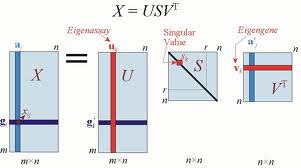
\includegraphics[width=0.6\textwidth]{IMAGES/svd.jpg}
\end{center}

\end{frame}


% ------------------------------------------
\begin{frame}
\frametitle{Singular value decomposition (svd)}

\begin{displaymath}
  A \;{\bf x} \;\;=\;\;  U D V^{\top} \; {\bf x} \;\; = \;\; 0
\end{displaymath}
\vspace{2mm}

We are not interested in the trivial solution ${\bf x = 0}$ but rather
all solution lying in the {\color{blue}{Null-space}} of the matrix
$A$. \\[3mm]

The singular values in the diagonal matrix $D$ specifies the
{\color{blue}{energy}} contained in each of the dimensions. Usually, these are
sorted in decreasing order. \\[3mm]

Often, due to noise all singular values $\sigma_i > 0$.  If we know
that $A$ should be singular may find the closest such matrix by
zeroing out the smallest singular value. \\[3mm]

We get the solution to $A {\bf x} = {\bf 0}$ as the last column of
$V$. In MATLAB: \\[3mm]

\texttt{
[U,D,V] = svd(A);  x = V(:,end);  
} 

Notice that $||x|| = 1$
\end{frame}




%-------------------------------------------------------------------
\begin{frame}
\frametitle{Camera calibration continued}
\begin{itemize}
\item Given 6 points $(x,y)$ projected from 6 known 3D points
         $(X,Y,Z)$ we can solve for the camera matrix elements $m_{ij}$. \\[5mm]
\item In practise many more than 6 points are preferred to cancel
          noise. \\[5mm] 
\item From the 12 elements $m_{ij}$ it is possible to recover all 11 
          parameters $f_x$, $f_y$, $\alpha$, $\beta$, $\gamma$, etc. \\[5mm]
\item There exist more advanced calibration methods than the shown 
          linear calibration. 
\end{itemize}

\end{frame}



%-------------------------------------------------------------------
\begin{frame}
  \begin{center}
    {\color{blue}{\Huge QUESTIONS ?}}
  \end{center}
 \end{frame}






% ----------------------------------------------------------------
% \begin{frame}
%   \frametitle{Assignment 4 - details}
%   \begin{itemize}
%   \item The assignment consists in implementing a prototypical Content
%    Based Image Retrieval System \\[5mm]
%  \item Five parts:
%    \begin{enumerate}
%     \item Select and prepare the data you want to work with \\[3mm]
%      \item Gather descriptors in training and test image data set \\[3mm]
%      \item Construct codebook using k-means and Bag-Of-Words \\[3mm]
%      \item Project test images onto codebook, and generate BoW \\[3mm]
%    \item Retrieve according to similarity measure
%    \end{enumerate}
%  \end{itemize}
% \end{frame}

%-------------------------------------------------------------------
% \begin{frame}
% \frametitle{What descriptors}
%  \begin{itemize}
%     \item   You are advised to use SIFT features
%     \item   Few versions of SIFT include color. You may miss a lot of
%       information. 
%     \item   You may include color histograms etc. but
%     \item   Advise: Keep it simple%
% \end{itemize}
% \end{frame}

 
 %-------------------------------------------------------------------
% \begin{frame}
%   \frametitle{Training and testing}
%   \begin{itemize}
%   \item Download Caltech-101 image database (131 MB) with 101
%     categories or the newer Caltech-256 base (1.2 GB) \\[5mm]
%   \item Split data into two parts: Training data [say 70-80\%] and test
%      [say 20-30 \%]. Don't look at the test data before  testing \\[5mm]
%    \item During development you may split the training data into a
%     construction part [say 80\%] and an validation part [say 20\%].\\[5mm]
%   \item Never use the test set for tuning ! 
%  \end{itemize}
% \end{frame}


%-------------------------------------------------------------------
% \begin{frame}
%  \frametitle{What error ?}
%  \begin{itemize}
%   \item Error on training data versus error on test data \\[5mm]
%   \item What if the training error is less than the test error? \\[5mm]
%%   \pause
%   \item Overfitting is a serious problem.  Often caused by using too
%     few training data (or too complicated model) \\[5mm]
%   \item We want to generalize in order to retrieve/classify new data
%  \end{itemize}
%  \end{frame}


 
%-------------------------------------------------------------------
% \begin{frame}
% \frametitle{Cross-validation}
%  \begin{itemize}
%   \item Divide data into say 10 sets (10-fold CV) \\[5mm]
%   \item Train on all but one set that is used testing \\[5mm]
%   \item Retrain and test on all possible combinations \\[5mm]
%   \item Compute the average test error
% \end{itemize}
%  \end{frame}


%-------------------------------------------------------------------
% \begin{frame}
%  \frametitle{How to report}
%  \begin{itemize}
%   \item Amount: {\color{blue}{8 pages}} including everything: 
%     Try to be concise, structured etc. Keep text less than 3-4 pages \\[5mm]
%   \item Discussion: This is the most important part \\[5mm]
%    \item Tables: Remember to tell me what I should notice \\[5mm]
%   \item Figures: Remember axis labels etc.  What should I see? \\[5mm]
%   \item Images: Don't show them too small. What should I see? \\[5mm]
%   \item Explanations: Don't expect me to guess what you mean or see
%     yourself \\[5mm]
%   \item {\color{blue}{ERROR ANALYSIS}}: Explain what you think may
%     cause observed errors or unexpected behaviour 
%   \end{itemize}
%   \end{frame}


%-------------------------------------------------------------------
% \begin{frame}
%  \begin{center}
%    {\color{blue}{\Huge QUESTIONS ?}}
%  \end{center}
%  \end{frame}





%-------------------------------------------------------------------
\begin{frame}
  \frametitle{Next time}

  Next time, our first meeting in 2022, we will continue with stereo
  analysis, multi view geometry and may be a bit about image
  stitching.
  
  \begin{center}
    
\includegraphics[width=0.8\textwidth]{IMAGES/MerryChristmas.jpg}
  \end{center}


 \end{frame}




% ---------------------------------
% Class evaluation ???
% \begin{frame}
%   \frametitle{Midway Class Evaluation}
%
% {\color{blue}{
% Traditional class evaluation difficult to do online.
% Instead, I will ask you to fill out the Midway-evaluation
% at Absalon.}} \\[4mm]
%  
% \begin{itemize}
% \item What do you think of the course so far ?
% \item Is there anything we never must do again ?
% \item What worked really well ?
% \item Given the CoVid19 situation, how may we improve ?
% \end{itemize}
% \end{frame}


% \begin{frame}
%   \frametitle{Possible questions}
%   \begin{itemize}
%%   \item Does the course live up to the course description / learning outcome?
%   \item Does the course live up to your expectations?
%   \item Do you like the selected topics?
%   \item How are the assignments?
%   \item How are the questionnaires?
%   \item How are the lectures/exercises?
%   \item Do you get sufficient feedback?
%   \item Do you like the textbook (Forsyth and Ponce)?
%   \item What has been most easy and most difficult ?
%   \item Anything else?
%   \end{itemize}
%   \vspace{5mm}
%
%   Please fill out the evaluation (under Quizzes), now or before Friday
%   afternoon. 
% \end{frame}





\end{document}


